\documentclass[12pt]{article}
\usepackage{amsmath}
\usepackage{amssymb,amsfonts,amsthm}
\usepackage{tikz,color,pgf,graphicx,url}
\usetikzlibrary{calc}
\usetikzlibrary{decorations.pathreplacing}
\usepackage{xcolor}

\begin{document}

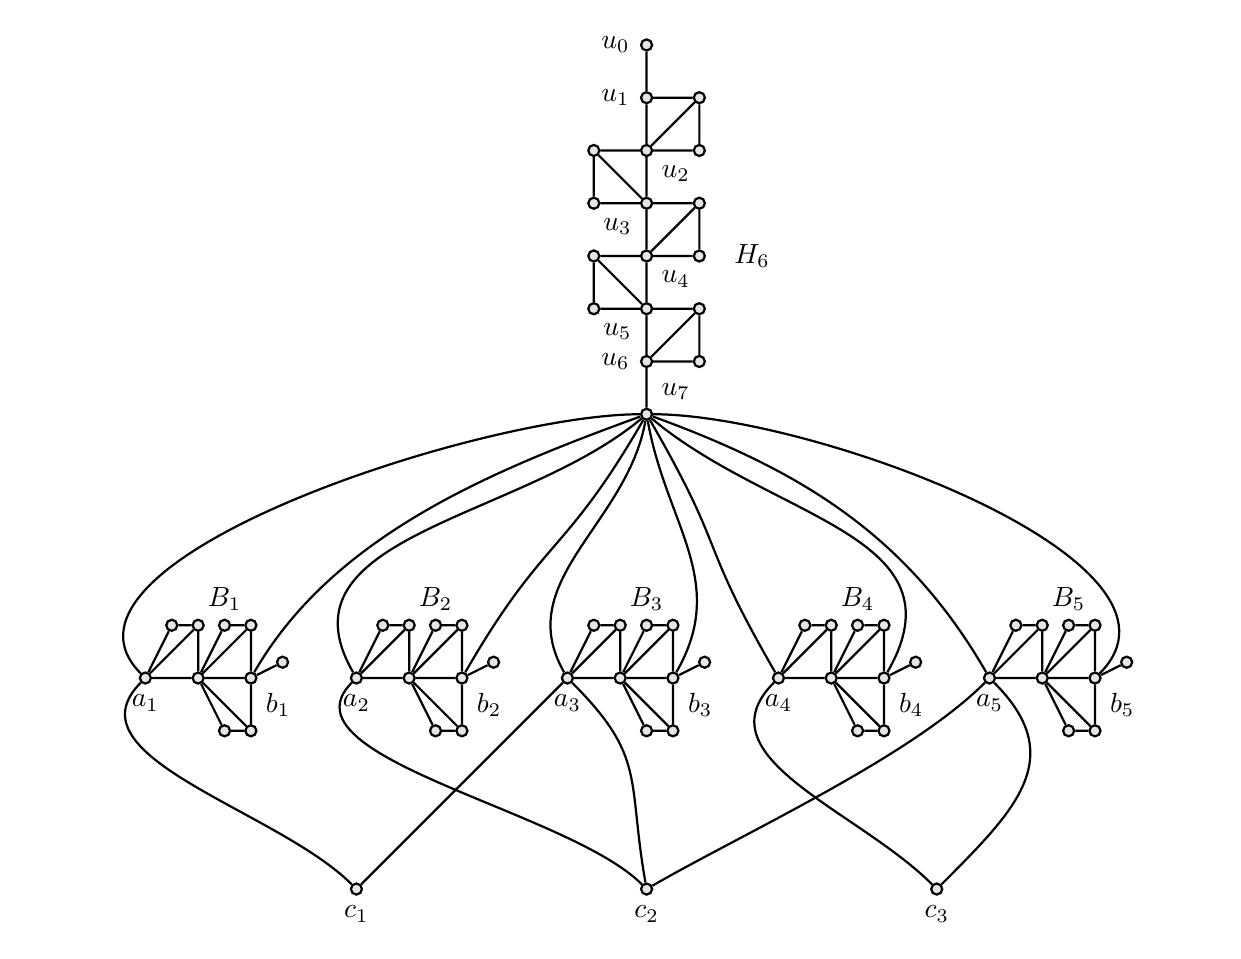
\begin{tikzpicture}[thick, scale = 0.67]
	% Define style for nodes
	\tikzstyle{vert}=[circle, draw, fill=black!10, inner sep=0pt, minimum width=4pt]

	\foreach \x in {1,2,3,4,5}{
		\node (k\x) at (4*\x - 4 +1.5,1.5) {$B_{\x}$};
		\node[vert, label=below: {$a_{\x}$}] (a\x) at (4*\x - 4 +0,0) {};
		\node[vert] (e\x) at (4*\x - 4+1,0) {};
		\node[vert, label=below right: {$b_{\x}$}] (b\x) at (4*\x - 4+2,0) {};
		\node[vert] (d\x) at (4*\x - 4+2.6,0.3) {};

		\node[vert] (h\x) at (4*\x - 4+1,1) {};
		\node[vert] (k1\x) at (4*\x - 4+0.5,1) {};

		\node[vert] (f1\x) at (4*\x - 4+2,1) {};
		\node[vert] (g1\x) at (4*\x - 4+1.5,1) {};

		\node[vert] (f2\x) at (4*\x - 4+2,-1) {};
		\node[vert] (g2\x) at (4*\x - 4+1.5,-1) {};


		\draw (a\x) -- (e\x) -- (b\x) -- (d\x);
		\draw (a\x) -- (h\x) -- (e\x) -- (f1\x) -- (b\x) -- (f2\x) -- (e\x) -- (g1\x) -- (f1\x);
		\draw (e\x) -- (g2\x) -- (f2\x);
		\draw (h\x) -- (k1\x) -- (a\x);	
	}

	\node (h) at (11.5,8) {$H_6$};
	\node[vert, label=above right: {$u_7$}] (u0) at (9.5,5) {};
	\node[vert, label=left: {$u_6$}] (u1) at (9.5,6) {};
	\node[vert, label=below left: {$u_5$}] (u2) at (9.5,7) {};
	\node[vert, label=below right: {$u_4$}] (u3) at (9.5,8) {};
	\node[vert, label=below left: {$u_3$}] (u4) at (9.5,9) {};
	\node[vert, label=below right: {$u_2$}] (u5) at (9.5,10) {};
	\node[vert, label=left: {$u_1$}] (u6) at (9.5,11) {};
	\node[vert, label=left: {$u_0$}] (u7) at (9.5,12) {};
	\node[vert] (x1) at (10.5,6) {};
	\node[vert] (y1) at (10.5,7) {};
	\node[vert] (x2) at (8.5,7) {};
	\node[vert] (y2) at (8.5,8) {};
	\node[vert] (x3) at (10.5,8) {};
	\node[vert] (y3) at (10.5,9) {};
	\node[vert] (x4) at (8.5,9) {};
	\node[vert] (y4) at (8.5,10) {};
	\node[vert] (x5) at (10.5,10) {};
	\node[vert] (y5) at (10.5,11) {};

	\draw (u0) -- (u1) -- (u2) -- (u3) -- (u4) -- (u5) -- (u6) -- (u7);
	\draw (y1) -- (u1) -- (x1) -- (y1) -- (u2);
	\draw (y2) -- (u2) -- (x2) -- (y2) -- (u3);
	\draw (y3) -- (u3) -- (x3) -- (y3) -- (u4);
	\draw (y4) -- (u4) -- (x4) -- (y4) -- (u5);
	\draw (y5) -- (u5) -- (x5) -- (y5) -- (u6);

	\draw (u0) to[out=180,in=135,distance=3cm] (a1);
	\draw (u0) to[out=-160,in=60,distance=3cm] (b1);
	\draw (u0) to[out=-140,in=120,distance=3cm] (a2);
	\draw (u0) to[out=-120,in=60,distance=3cm] (b2);

	\draw (u0) to[out=-100,in=120,distance=2cm] (a3);
	\draw (u0) to[out=-80,in=60,distance=2cm] (b3);

	\draw (u0) to[out=-60,in=120,distance=3cm] (a4);
	\draw (u0) to[out=-40,in=60,distance=3cm] (b4);
	\draw (u0) to[out=-20,in=120,distance=3cm] (a5);
	\draw (u0) to[out=0,in=45,distance=3cm] (b5);

	\node[vert, label=below:{$c_1$}] (c1) at (4,-4) {};
	\node[vert, label=below:{$c_2$}] (c2) at (9.5,-4) {};
	\node[vert, label=below:{$c_3$}] (c3) at (15,-4) {};

	\draw (c1) to[out=135,in=-135,distance=2cm] (a1);
	\draw (c1) to[out=45,in=-135,distance=2cm] (a3);

	\draw (c2) to[out=135,in=-135,distance=2cm] (a2);
	\draw (c2) to[out=100,in=-45,distance=2cm] (a3);
	\draw (c2) to[out=30,in=-135,distance=2cm] (a5);

	\draw (c3) to[out=135,in=-135,distance=2cm] (a4);
	\draw (c3) to[out=45,in=-45,distance=2cm] (a5);		
\end{tikzpicture}

\end{document}